\documentclass[11pt,a4paper]{article}

\usepackage[utf8]{inputenc}
\usepackage[T1]{fontenc}
\usepackage[brazil]{babel}
\usepackage[margin=2.5cm]{geometry}
\usepackage{graphicx}
\usepackage{booktabs}
\usepackage{amsmath}
\usepackage{float}
\usepackage[hidelinks]{hyperref}

\graphicspath{{../}{../Resultados/}}

\title{PRJ-23 -- Aircraft Preliminary Design\\
       \Large Homework 02 -- Otimização}
\author{Equipe Ararinha\\ \small (preencher nomes dos integrantes)}
\date{Setembro de 2026}

\begin{document}

\maketitle

\section{Otimização da aeronave default}

O problema definido no roteiro --- minimizar o MTOW da \texttt{standard\_airplane}
(\texttt{fokker100}) com respeito a $7 \le AR_w \le 12$ e
$80 \le S_w \le 120~\mathrm{m^2}$, sujeito a $b_w \le 30$~m --- foi resolvido
com o SLSQP do \texttt{scipy.optimize.minimize}, com gradientes por diferenças
finitas e partida em $AR_w = 7{,}5$, $S_w = 90~\mathrm{m^2}$. As variáveis de
projeto foram normalizadas pelos valores iniciais.

\begin{table}[H]
\centering
\caption{Resultados da otimização da aeronave default.}
\begin{tabular}{lcccc}
\toprule
 & $AR_w$ & $S_w$ [m$^2$] & MTOW [kgf] & $b_w$ [m] \\
\midrule
Ponto de partida & 7{,}500  & 90{,}00 & 43.066{,}6 & 25{,}98 \\
Ponto ótimo      & 10{,}522 & 84{,}88 & 41.879{,}7 & 29{,}89 \\
\bottomrule
\end{tabular}
\end{table}

\begin{enumerate}
\item Os resultados estão na tabela acima.
\item A melhoria relativa do objetivo foi de \textbf{2{,}756\,\%}.
\item Foram 33 chamadas da função objetivo (\texttt{nfev}), correspondendo a
      68 execuções do \texttt{analyze} (objetivo e restrição em varreduras
      separadas de diferenças finitas), em 11 iterações do SLSQP.
\item \textbf{O ótimo não é restringido}: é um ponto interior. A envergadura
      final, $b_w = 29{,}89$~m, fica aquém do limite de 30~m
      ($g = -3{,}8\cdot10^{-3}$, inativa), nenhum bound está ativo e a norma
      do gradiente do objetivo no ótimo é $\|\nabla f\| \approx 7\cdot10^{-6}$.
      A condição de otimalidade se reduz a $\nabla f = 0$, sem contribuição de
      multiplicadores, como se visualiza no espaço de projeto da
      Fig.~\ref{fig:fokker_espaco}.
\end{enumerate}

\begin{figure}[H]
\centering

\includegraphics[width=0.75\textwidth]{fokker100_historico.png}
\caption{Histórico da otimização da aeronave default.}
\label{fig:fokker_hist}
\end{figure}

\begin{figure}[H]
\centering

\includegraphics[width=0.75\textwidth]{fokker100_espaco_projeto.png}
\caption{Espaço de projeto ($AR_w \times S_w$), trajetória do otimizador e
         restrição de envergadura. O ótimo (azul) é interior.}
\label{fig:fokker_espaco}
\end{figure}

\section{Otimização da aeronave da equipe}

\subsection{Definição do problema e escolha das variáveis (pergunta 1)}

Minimizar $W_0$ da aeronave da equipe (configuração final do PRJ-22,
\texttt{my\_airplane}) com respeito a 8 variáveis de projeto:

\begin{table}[H]
\centering
\caption{Variáveis de projeto, valores iniciais e limites.}
\begin{tabular}{lccc}
\toprule
DV & inicial & limite inferior & limite superior \\
\midrule
$AR_w$            & 8{,}00   & 7{,}00   & 12{,}00 \\
$x_{r,w}$ [m]     & 17{,}00  & 14{,}00  & 20{,}00 \\
$S_w$ [m$^2$]     & 390{,}0  & 330{,}0  & 460{,}0 \\
$\Lambda_w$ [rad] & 0{,}580  & 0{,}400  & 0{,}700 \\
$x_{mlg}$ [m]     & 31{,}00  & 28{,}00  & 35{,}00 \\
$(t/c)_{r,w}$     & 0{,}180  & 0{,}120  & 0{,}240 \\
$z_{lg}$ [m]      & $-5{,}75$ & $-7{,}50$ & $-4{,}50$ \\
$y_{mlg}$ [m]     & 5{,}50   & 4{,}00   & 9{,}00  \\
\bottomrule
\end{tabular}
\end{table}

As cinco primeiras variáveis da asa controlam os principais trade-offs de
$W_0$: arrasto induzido ($AR_w$), área molhada e carga alar ($S_w$), arrasto
de onda ($\Lambda_w$, $t/c$), peso estrutural da asa ($t/c$, $AR_w$, $S_w$) e
balanceamento/tanque ($x_{r,w}$). As três variáveis de trem de pouso
($x_{mlg}$, $z_{lg}$, $y_{mlg}$) não afetam diretamente o objetivo no modelo
(o peso do trem no \texttt{designTool} depende apenas de $W_0$), mas são
indispensáveis para manter viáveis as restrições de solo
(\emph{tipback}, \emph{tailstrike}, \emph{overturn}, frações do triquilho)
enquanto a asa muda de posição e forma. Todas as DVs e restrições foram
normalizadas pelos valores de referência, como recomendado no roteiro ---
sem isso a jacobiana misturaria escalas de $5\cdot10^{-2}$ a $4\cdot10^{2}$.

\subsection{Restrições adicionadas (pergunta 2)}

Além das restrições mínimas do roteiro, foram adicionadas:
\begin{itemize}
\item $\texttt{T0req} \le 1$: o empuxo requerido em todas as condições de
      dimensionamento (decolagem, cruzeiros e gradientes FAR~25) não pode
      exceder o empuxo máximo dos motores selecionados;
\item $\texttt{vt\_fit} \le 1$: a corda da raiz da empenagem vertical deve
      terminar dentro do comprimento da fuselagem;
\item $\texttt{mlg\_fit} \le 1$: o trem principal deve ficar sob a asa
      (à frente do bordo de fuga na estação lateral do trem). O bordo de fuga
      é obtido interpolando o bordo de ataque entre a raiz e a ponta
      ($x_{t,w}$ do \texttt{designTool}, que já embute o termo de $1/4$ de
      corda, pois $\Lambda_w$ é medido a $1/4$ de corda);
\item $\texttt{ground\_clearance} \ge 0{,}5$~m: folga entre o fundo da nacele
      e o solo --- necessária porque $z_{lg}$ é variável de projeto e seu
      bound superior permitiria a nacele abaixo do solo;
\item Limites geométricos na interpretação estrita do Anexo 14
      (``up to but not including''): $b_w \le 64{,}9$~m e trilha do trem
      $\le 13{,}9$~m (código E); altura da empenagem $\le 20$~m (FAA ADG~V).
\end{itemize}

\subsection{Comparação inicial \(\times\) otimizado (pergunta 3)}

\begin{table}[H]
\centering
\caption{Variáveis de projeto e objetivos: baseline (PRJ-22) $\times$ ótimo.}
\begin{tabular}{lccc}
\toprule
 & inicial & otimizado & variação \\
\midrule
$AR_w$            & 8{,}000  & 9{,}800  & $+22{,}5\,\%$ \\
$x_{r,w}$ [m]     & 17{,}000 & 16{,}011 & $-5{,}8\,\%$  \\
$S_w$ [m$^2$]     & 390{,}00 & 353{,}67 & $-9{,}3\,\%$  \\
$\Lambda_w$ [rad] & 0{,}580  & 0{,}611  & $+5{,}3\,\%$  \\
$x_{mlg}$ [m]     & 31{,}000 & 29{,}263 & $-5{,}6\,\%$  \\
$(t/c)_{r,w}$     & 0{,}180  & 0{,}209  & $+16{,}3\,\%$ \\
$z_{lg}$ [m]      & $-5{,}750$ & $-6{,}025$ & $+4{,}8\,\%$ \\
$y_{mlg}$ [m]     & 5{,}500  & 6{,}950  & $+26{,}4\,\%$ \\
\midrule
$W_0$ [kgf] & 306.745{,}2 & 290.117{,}1 & $\mathbf{-5{,}42\,\%}$ \\
$W_f$ [kgf] & 122.743{,}5 & 111.036{,}5 & $-9{,}54\,\%$ \\
\bottomrule
\end{tabular}
\end{table}

\begin{table}[H]
\centering
\caption{Restrições no ponto inicial e no ótimo ($g$ normalizada $\ge 0$;
         ativa se $|g| < 10^{-4}$).}
\small
\begin{tabular}{lcccc}
\toprule
restrição & inicial & otimizado & limite & estado \\
\midrule
\texttt{deltaS\_wlan}      & 0{,}300 & 0{,}257 & $\ge 0$ & \\
\texttt{SM\_fwd}           & 0{,}270 & 0{,}300 & $\le 0{,}30$ & \textbf{ATIVA} \\
\texttt{SM\_aft}           & 0{,}083 & 0{,}050 & $\ge 0{,}05$ & \\
\texttt{frac\_nlg\_fwd}    & 0{,}160 & 0{,}126 & $\le 0{,}18$ & \\
\texttt{frac\_nlg\_aft}    & 0{,}108 & 0{,}062 & $\ge 0{,}03$ & \\
\texttt{alpha\_tipback} [$^\circ$]    & 27{,}72 & 15{,}00 & $\ge 15$ & \textbf{ATIVA} \\
\texttt{alpha\_tailstrike} [$^\circ$] & 10{,}12 & 10{,}00 & $\ge 10$ & \textbf{ATIVA} \\
\texttt{phi\_overturn} [$^\circ$]     & 51{,}76 & 45{,}73 & $\le 63$ & \\
\texttt{ground\_clearance} [m] & 0{,}750 & 1{,}025 & $\ge 0{,}5$ & \\
\texttt{tank\_excess}      & 0{,}012 & 0{,}000 & $\ge 0$ & \textbf{ATIVA} \\
$b_w$ [m]                  & 55{,}86 & 58{,}87 & $\le 64{,}9$ & \\
\texttt{mlg\_track} [m]    & 11{,}00 & 13{,}90 & $\le 13{,}9$ & \textbf{ATIVA} \\
\texttt{h\_tail} [m]       & 18{,}62 & 18{,}43 & $\le 20$ & \\
\texttt{T0req}             & 0{,}829 & 0{,}833 & $\le 1$ & \\
\texttt{vt\_fit}           & 0{,}967 & 0{,}981 & $\le 1$ & \\
\texttt{mlg\_fit}          & 1{,}013 & 1{,}000 & $\le 1$ & \textbf{ATIVA} \\
\bottomrule
\end{tabular}
\end{table}

Vale registrar que a baseline do PRJ-22 era \emph{inviável} em
\texttt{mlg\_fit}: o trem principal em $x = 31$~m ficava atrás do bordo de
fuga da asa ($\approx 30{,}6$~m na estação do trem). A otimização corrigiu
essa inconsistência.

\subsection{Otimizador (pergunta 4)}

SLSQP (\texttt{scipy}), com gradientes por diferenças finitas. O método é
adequado porque o problema é suave e de pequena dimensão (8 DVs), tem
restrições de desigualdade não lineares e bounds --- tratados nativamente
pelo SQP --- e a análise é barata ($\sim$7~ms) e determinística, o que torna
as diferenças finitas confiáveis. Métodos sem gradiente escalariam pior com
o número de variáveis, como visto em aula.

\subsection{Melhoria relativa (pergunta 5)}

$W_0$ caiu \textbf{5{,}42\,\%} ($-16{,}6$~t) e $W_f$ caiu $9{,}54\,\%$
($-11{,}7$~t) em relação à aeronave do PRJ-22.

\subsection{Custo computacional (pergunta 6)}

91 chamadas da função objetivo (\texttt{nfev}), 182 execuções do
\texttt{analyze}, 10 iterações do SLSQP, $\approx 0{,}6$~s de tempo total.

\subsection{Histórico da otimização (pergunta 7)}

\begin{figure}[H]
\centering
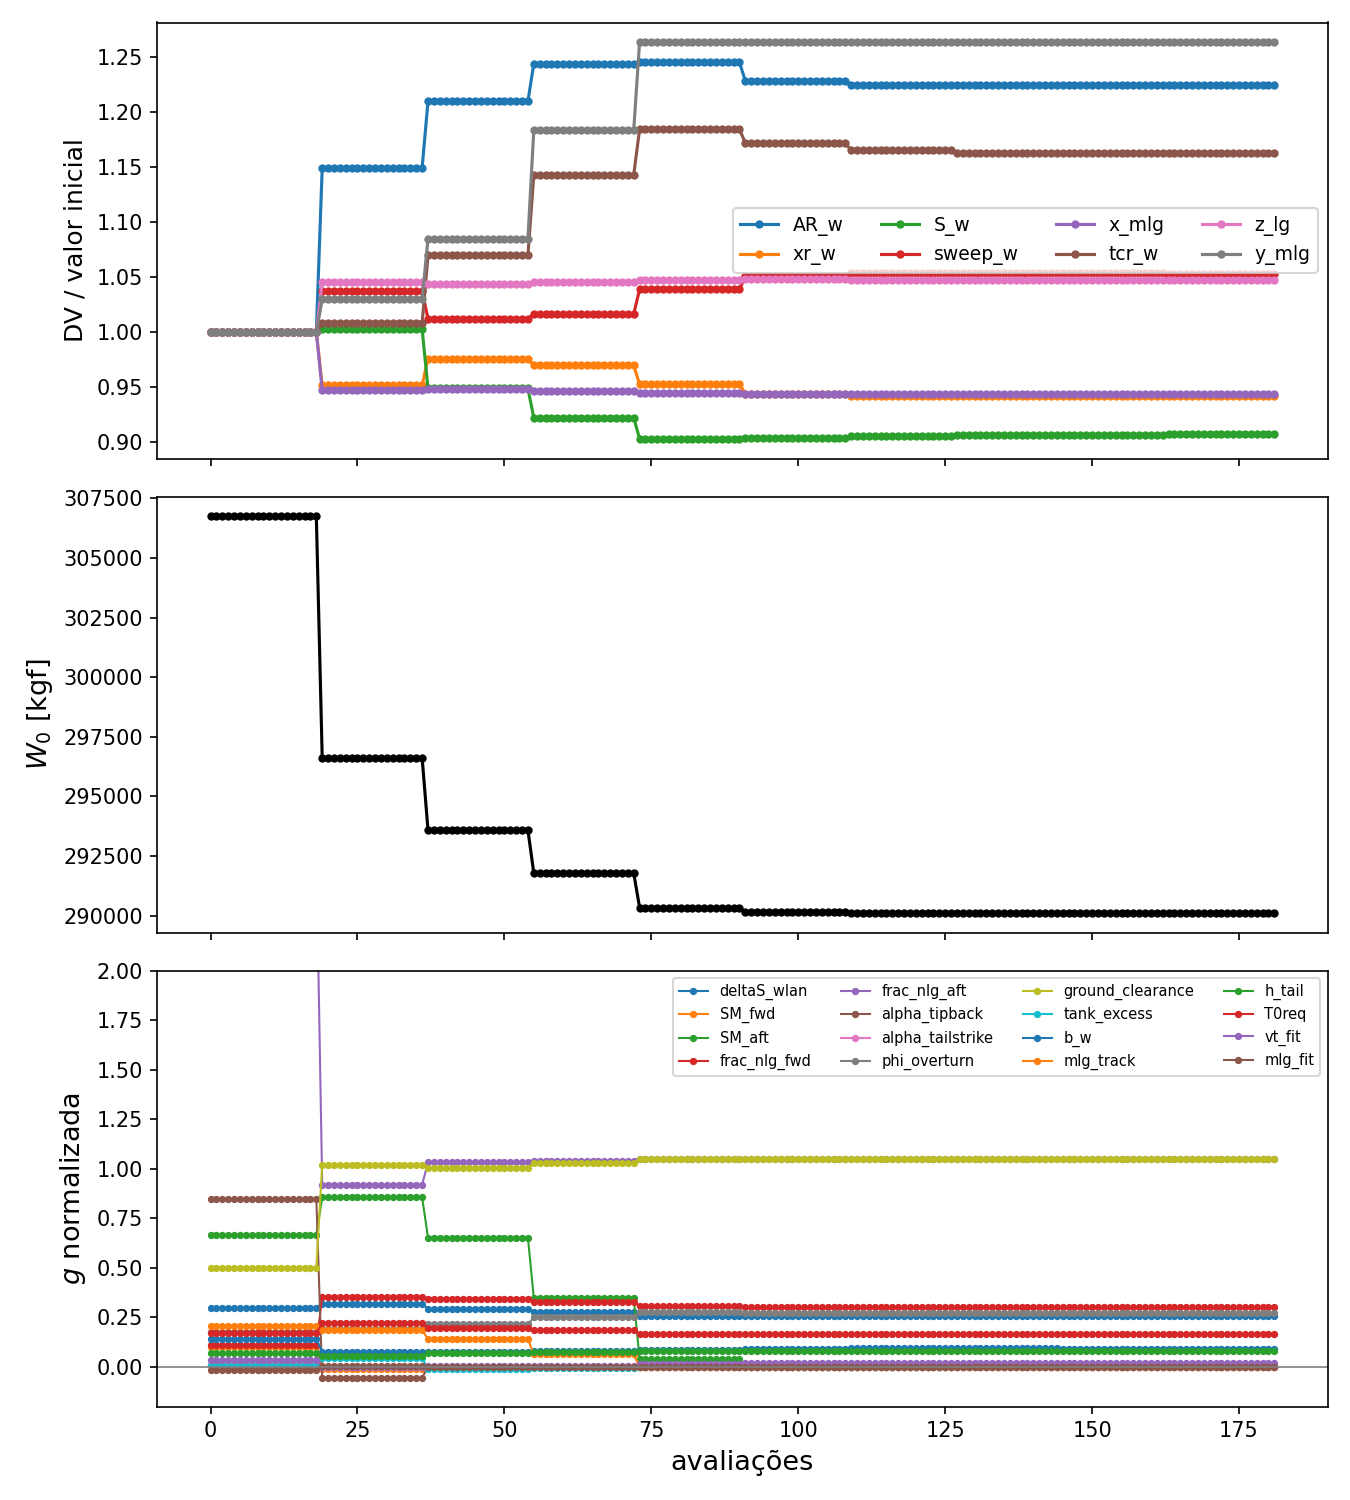
\includegraphics[width=0.95\textwidth]{equipe_geom_historico.png}
\caption{Histórico das variáveis de projeto (normalizadas), do objetivo e
         das restrições normalizadas.}
\label{fig:equipe_hist}
\end{figure}

\subsection{O ótimo é restringido? (pergunta 8)}

Sim. Seis restrições estão ativas no ótimo --- \texttt{SM\_fwd},
\texttt{alpha\_tipback}, \texttt{alpha\_tailstrike}, \texttt{tank\_excess},
\texttt{mlg\_track} e \texttt{mlg\_fit} --- e nenhum bound. A física do
resultado: $AR_w\uparrow$ e $S_w\downarrow$ reduzem arrasto induzido e área
molhada; a raiz mais espessa barateia a estrutura da asa mais esbelta com
pouca penalidade de onda (o enflechamento $+5\,\%$ compensa); o combustível
fecha justo (\texttt{tank\_excess} $=0$) e o CG dianteiro encosta em
$SM = 0{,}30$. O trem alarga até a trilha-limite de $13{,}9$~m porque a
estação mais externa da asa enflechada tem bordo de fuga mais recuado,
aliviando \texttt{mlg\_fit} e permitindo o trem mais atrás; \emph{tipback} e
\emph{tailstrike} ativas amarram $x_{mlg}$ e $z_{lg}$.

\subsection{Planformas (pergunta 9)}

\begin{figure}[H]
\centering
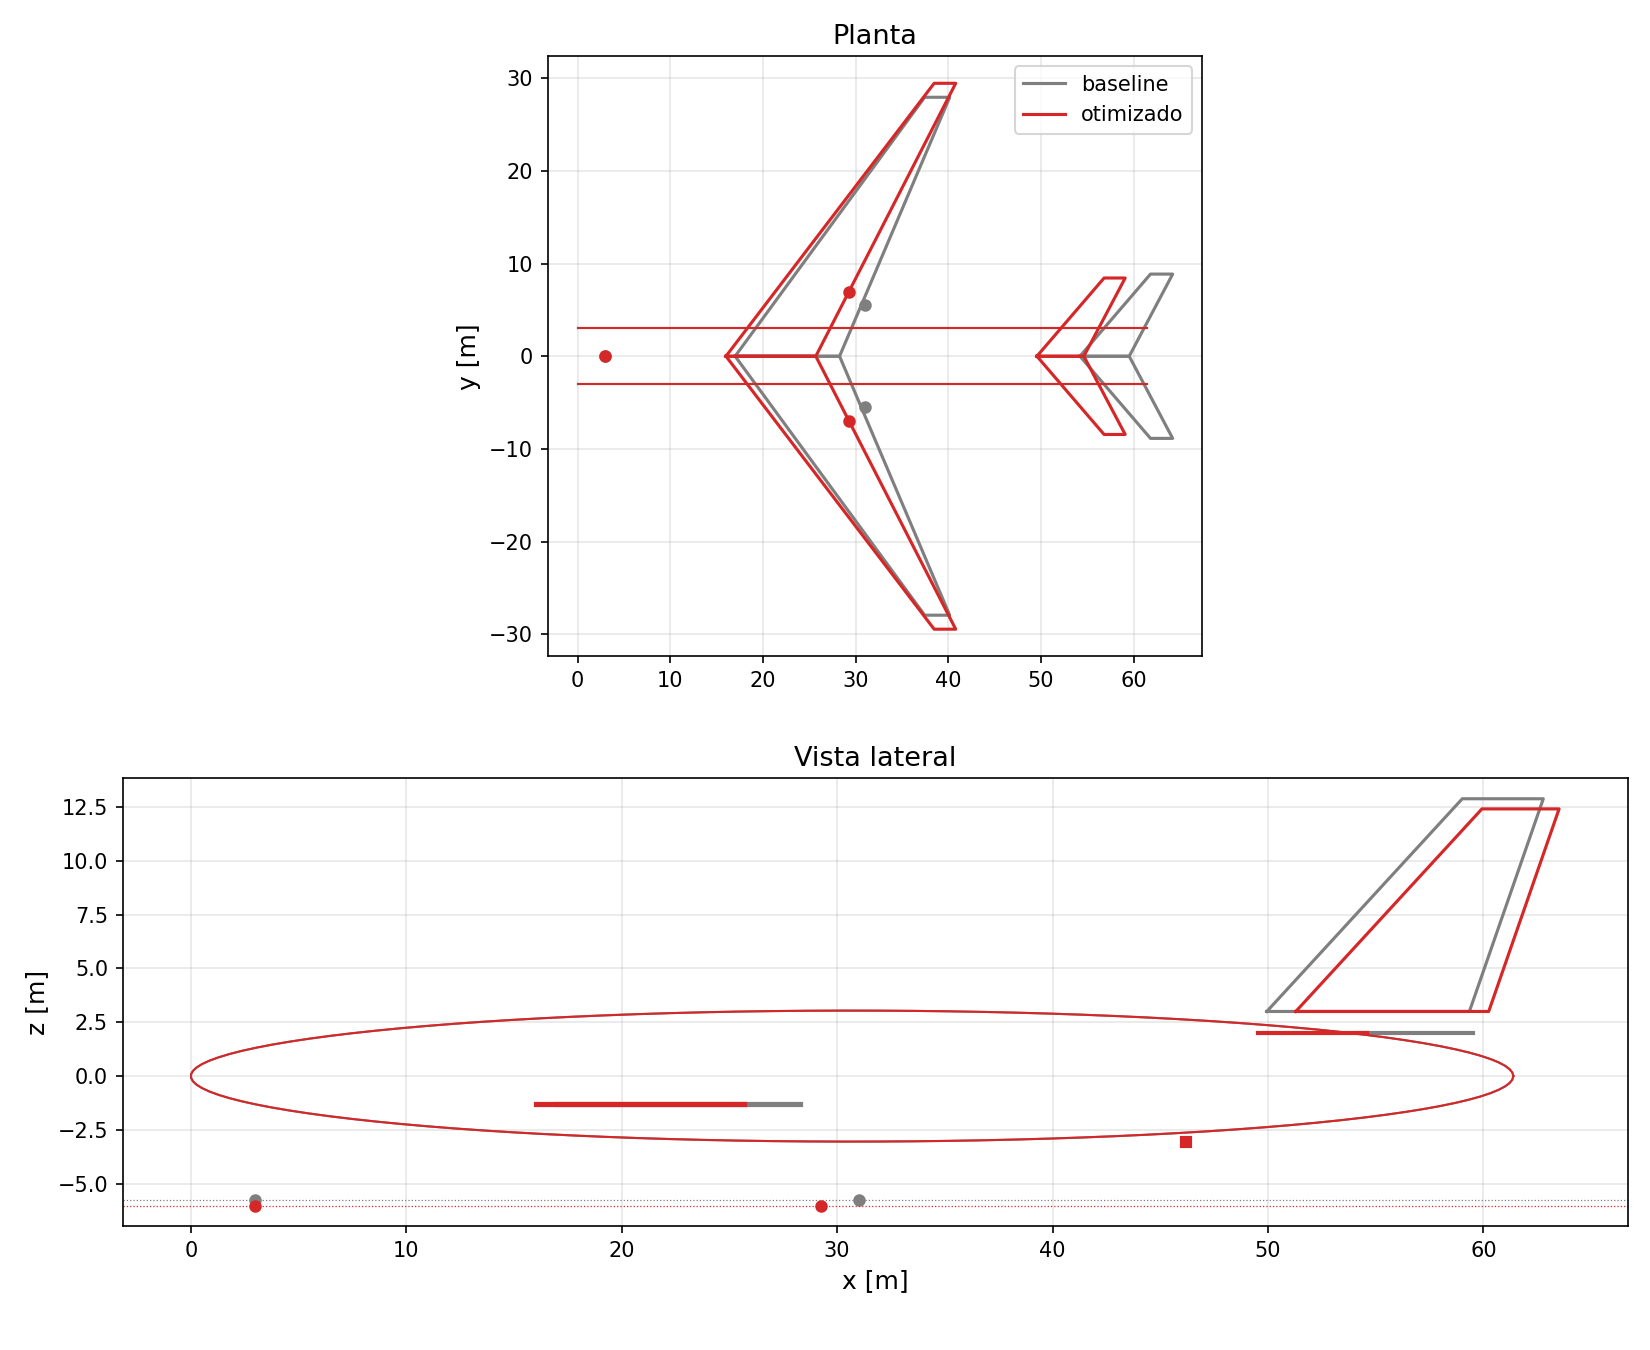
\includegraphics[width=0.95\textwidth]{equipe_geom_planformas.png}
\caption{Planta e vista lateral: baseline (cinza) $\times$ otimizada
         (vermelho).}
\label{fig:equipe_planformas}
\end{figure}

\section{Otimização multiobjetivo}

O problema da Seção~2 foi repetido minimizando simultaneamente $W_0$ e
$W_f$, com as mesmas 8 DVs e 16 restrições, usando o NSGA-II do
\texttt{pymoo} (nota: o \texttt{pymoo} considera viável $G \le 0$, sinal
oposto ao \texttt{scipy}). Avaliações em que a iteração de ponto fixo do
$W_0$ diverge (a população aleatória gera geometrias extremas) são
devolvidas como indivíduos fortemente inviáveis.

\subsection{Frente de Pareto (pergunta 1)}

\begin{figure}[H]
\centering

\includegraphics[width=0.8\textwidth]{equipe_moga_pareto.png}
\caption{Frente de Pareto $W_0 \times W_f$, com a baseline, os ótimos
         mono-objetivo (SLSQP) e as três aeronaves selecionadas.}
\label{fig:pareto}
\end{figure}

\subsection{Gerações e indivíduos (pergunta 2)}

\textbf{80 indivíduos por geração} e \textbf{200 gerações}
(16.000 execuções do \texttt{analyze}, $\approx 368$~s, semente 1),
com população inicial por hipercubo latino semeada com a baseline e os dois
ótimos mono-objetivo. A frente final tem 36 pontos.

\subsection{Verificação de convergência com a Seção 2 (pergunta 3)}

Os extremos da frente devem coincidir com os ótimos mono-objetivo do mesmo
problema: $\min W_0$ (SLSQP) $= 290.117{,}1$~kgf e $\min W_f$ (SLSQP)
$= 109.117{,}9$~kgf. Essa comparação é um teste objetivo de convergência:
uma rodada \emph{sem} sementes (pop.\ 60, 120 gerações) estagnou com o
extremo de mínimo $W_0$ em $293.379{,}9$~kgf --- $+1{,}12\,\%$ acima da
âncora, com a frente inteira dominada pelos dois pontos do SLSQP,
evidenciando não convergência. A rodada final fecha os extremos em
$+0{,}42\,\%$ ($W_0$) e $+0{,}77\,\%$ ($W_f$) das âncoras; o resíduo é
esperado do NSGA-II em ótimos ``de canto'' com várias restrições ativas,
que o método de gradiente resolve com precisão muito maior.

\subsection{Três aeronaves da frente (pergunta 4)}

\begin{table}[H]
\centering
\caption{Aeronaves selecionadas de regiões distintas da frente de Pareto.}
\begin{tabular}{lccccc}
\toprule
aeronave & $W_0$ [kgf] & $W_f$ [kgf] & $S_w$ [m$^2$] & $(t/c)_{r,w}$ & $AR_w$ \\
\midrule
A ($\min W_0$) & 291.327{,}7 & 110.938{,}4 & 364{,}2 & 0{,}202 & 9{,}66 \\
B (joelho)     & 291.750{,}4 & 110.033{,}7 & 369{,}9 & 0{,}193 & 9{,}72 \\
C ($\min W_f$) & 292.499{,}8 & 109.961{,}1 & 374{,}8 & 0{,}189 & 9{,}66 \\
\bottomrule
\end{tabular}
\end{table}

\begin{figure}[H]
\centering

\includegraphics[width=0.85\textwidth]{equipe_moga_planformas.png}
\caption{Planformas das três aeronaves selecionadas.}
\label{fig:moga_planformas}
\end{figure}

De A para C trocam-se $\approx 1{,}2$~t de MTOW por $\approx 1$~t de
combustível: a asa maior e mais fina voa mais eficiente (menos arrasto
induzido e de onda por unidade de área), ao custo de estrutura mais pesada.
Como $W_0$ e $W_f$ são apenas parcialmente conflitantes, a frente é estreita
e as planformas são quase idênticas --- o trade-off está na área e na
espessura, não na forma em planta. A escolha da equipe recairia sobre a
região do joelho (B), onde a troca marginal entre os objetivos é equilibrada.

\appendix
\section{Correções de modelagem feitas durante o trabalho}

Durante a revisão da otimização, duas correções foram aplicadas ao script:

\begin{enumerate}
\item \textbf{Bordo de fuga em \texttt{mlg\_fit}}: a fórmula original tratava
      $\Lambda_w$ como enflechamento de bordo de ataque, mas o
      \texttt{designTool} o define a $1/4$ de corda (termo
      $(c_r - c_t)/4$ no cálculo de $x_{t,w}$ em \texttt{geometry.py}).
      O bordo de fuga ficava subestimado em $\approx 0{,}45$~m e, com a
      restrição ativa, o ótimo pagava $\approx 2{,}9$~t de MTOW a mais
      ($293.064$ vs.\ $290.117$~kgf).
\item \textbf{Folga da nacele}: com $z_{lg}$ como variável de projeto, o
      bound superior ($-4{,}5$~m) permitiria o fundo da nacele
      ($z = -5{,}0$~m) abaixo do solo; a restrição
      $\texttt{ground\_clearance} \ge 0{,}5$~m elimina esse risco
      (no ótimo ela resulta inativa, com folga de $1{,}02$~m).
\end{enumerate}

\end{document}
